%%%%%% Verander de volgende lijnen niet %%%%%%%

\documentclass[12pt,a4paper,svgnames,oneside]{book}
\input{inputs/oplossingen-file-commandos.tex}
\initialiseer{inputs/oplossingen-alle.tmp}{inputs/oplossingen-zonder-ster.tmp}
\input{inputs/preamble-macro.tex}
\usepackage{amsmath}
\usepackage{hyperref}
\usepackage{subcaption}
\usepackage{tikz}
\usepackage{pgfplots,mathrsfs}
\usepackage{marginnote}
\usepackage[bottom]{footmisc}
\usepackage{schemabloc}
\usetikzlibrary{circuits}
\usepackage{verbatim}
\usetikzlibrary{arrows, decorations.markings}
\usepackage{soul}

\usepackage{array}

\newcolumntype{L}[1]{>{\raggedright\let\newline\\\arraybackslash\hspace{0pt}}p{#1}}
\newcolumntype{C}[1]{>{\centering\let\newline\\\arraybackslash\hspace{0pt}}p{#1}}
\newcolumntype{R}[1]{>{\raggedleft\let\newline\\\arraybackslash\hspace{0pt}}p{#1}}

\newcommand{\opdrachteindbalk}{
	\begin{tikzpicture}
	\fill[fill=fac-color-orange] (0,\streepdikte/2) rectangle (\textwidth,-\streepdikte/2);
	\end{tikzpicture}}

\sethlcolor{lightgray}

\begin{document}
\addtocounter{page}{-1}

%% We beginnen met het logo te defini\"{e}ren: de syntax is
%% \renewcommand{\filenaamlogo}{inputs/....}
%% waarbij je .... vervangt door de filenaam van het logo. Alvast drie beschikbare mogelijkheden zijn:
%% \renewcommand{\filenaamlogo}{inputs/kubus-wetenschappen.png}
%% \renewcommand{\filenaamlogo}{inputs/esat-logo.pdf}


\renewcommand{\filenaamlogo}{inputs/logo-innovationlab.png}

%% In de volgende lijn importeer je (in pdf) de frontpagina. Die maken we apart aan in een uniforme stijl. Er worden andere kleuren gebruikt voor de leerlingenbundels en voor de lerarenbundels.
%% Je kan de volgende regel veranderen in
%% \includepdf{inputs/voorbeeld-cover-vooraan-lkr.pdf}

\includepdf{inputs/frontcover.pdf}

%% Verander de volgende lijn niet.

\tableofcontents
%%%%%%%%%%%%%%%%%%%%%%%%%%%%%%%%%%%%%%%%%%%%%%%%%%%%%%%%%%%%%%%%%%%%%%%%%
%%%%%%%%%%%%%%%%%%%%%%%%%%%%%%%%%%%%%%%%%%%%%%%%%%%%%%%%%%%%%%%%%%%%%%%
%%%%%%%%%%%%%%%%%%%%%%%%%%%%%%%%%%%%%%%%%%%%%%%%%%%%%%%%%%%%%%%%%%%%%%%
\deelmetoef{Module 1}{Inleiding}{Module 1. Inleiding}{Oplossingen module 1}{Oplossingen module 1}
%%%%%%%%%%%%%%%%%%%%%%%%%%%%%%%%%%%%%%%%%%%%%%%%%%%%%%%%%%%%%%%%%%%%%%%
%%%%%%%%%%%%%%%%%%%%%%%%%%%%%%%%%%%%%%%%%%%%%%%%%%%%%%%%%%%%%%%%%%%%%%%

\begin{samenvatting}
Tijdens dit project maken we een smartphone app waarmee je je hartslag kan meten. Waarom het belangrijk is af en toe je hartslag te meten en waarom we dit met een app willen doen, wordt hierna uitgelegd. Daarna bekijken we wat een hartslag nu precies is, en hoe we die met onze smartphone kunnen meten.
\end{samenvatting}
%

%%%%%%%%%%%%%%%%%%%%%%%%%%%%%%%%%%%%%%%%%%%%%%%%%%%%%%%%%%%%%%%%%%%%%%%
\section{Wat en waarom?}
\label{sec:Mod1_Sec1}
%%%%%%%%%%%%%%%%%%%%%%%%%%%%%%%%%%%%%%%%%%%%%%%%%%%%%%%%%%%%%%%%%%%%%%%
%
De hartslag duidt aan hoe vaak je hart klopt per minuut. Tijdens het sporten is het belangrijk je hartslag in het oog te houden. Een te hoge hartslag wijst op een te hoge inspanning, en kan mogelijks gevaarlijk zijn. Bovendien kan een (te) hoge hartslag in rust wijzen op aandoeningen zoals een overactieve schildklier, bloedarmoede of bloedverlies, een longaandoening enz. Regelmatig je hartslag controleren is dus de boodschap.

Om je hartslag te meten wordt meestal gebruik gemaakt van een bloeddrukmeter.

\begin{minipage}{.5\linewidth}
	\gewonefiguur{width=\linewidth}{module1/patient}
\end{minipage} 
\begin{minipage}{.5\linewidth}
	\gewonefiguur{width=\linewidth}{module1/hartslagmonitor}
\end{minipage} 

Een bloeddrukmeter is een gespecialiseerd toestel dat meestal enkel een dokter of iemand met hartklachten ter beschikking heeft. Bovendien is het nogal omslachtig een bloeddrukmeter tijdens het sporten mee te nemen, gezien dit niet echt een draagbaar toestel is.

\gewonefiguur{width=.5\linewidth}{module1/lopermethartslagmeter}

Naast een bloeddrukmeter kan ook een hartslagmeter gebruikt worden om de hartslag te meten. 

\begin{minipage}{.5\linewidth}
	\gewonefiguur{width=\linewidth}{hartslagmeter}
\end{minipage} 
\begin{minipage}{.5\linewidth}
	\gewonefiguur{width=\linewidth}{module1/loper-met-dure-loopband}
\end{minipage} 

In tegenstelling tot een bloeddrukmeter kan je een hartslagmeter wel makkelijk meenemen bij het sporten en geeft ook real time feedback. Maar wellicht ligt de aanschaf van een hartslagmeter niet binnen het budget van elke leerling of student?

Daarom bouwen wij in dit project onze eigen smartphone app, waarmee we snel, eenvoudig en redelijk accuraat onze hartslag kunnen meten, zonder nood aan gespecialiseerde toestellen.

\gewonefiguur{width=.5\linewidth}{module1/loper}

\section{De hartslag}
\label{sec:Mod1_Sec2}

Je hart is een spier, die samentrekt om je bloed in je lichaam rond te pompen. De hartslag is de pompbeweging van je hart. In de volksmond is de hartslag ook het aantal samentrekkingen van je hart per minuut, of anders gezegd het aantal keer dat je hart klopt per minuut.

De hartslag van een volwassene varieert tussen 60 en 100 slagen per minuut. De maximale hartslag is de hoogste hartslag die je lichaam aan kan gedurende fysische activiteit. De maximale hartslag varieert naargelang je leeftijd en kan berekend worden met de volgende vuistregel

\begin{equation*}
MH = 220-LT
\end{equation*}

met volgende notatie:
\begin{itemize}
	\item MH: maximale hartslag met als eenheid slagen per minuut of \textquotedblleft beats per minute \textquotedblright (kortweg: \emph{bpm}). 
	Dit noteren we als MH [bpm].
	\item LT [jaar]: leeftijd
\end{itemize}

Het wordt aangeraden tijdens het sporten je hartslag tussen 55 en 85\% van je maximale hartslag te houden. 

Voor een volwassene van 20 jaar oud is het aangeraden hartslagbereik tijdens het sporten dus tussen 110 en 170 bpm.

\begin{table}
	\centering
	\begin{tabular}{c|ccc}
		LT & MH & 0,55*MH & 0,85*MH \\
		\hline
		20 & 200 & 110 & 170 \\
		50 & 170 & 94 & 145 
	\end{tabular}
\end{table}

\begin{oef}
Bereken de maximale hartslag en het ideale hartslagbereik tijdens het sporten van een volwassene van 
\begin{itemize}
	\item 18 jaar
	\item 30 jaar
	\item 65 jaar
\end{itemize}
\end{oef}
\oplos{\begin{itemize}
		\item $MH_{18}=202$ en hartslagbereik tussen 111,1 en 171,7
		\item $MH_{30}=190$ en hartslagbereik tussen 104,5 en 161,5
		\item $MH_{65}=155$ en hartslagbereik tussen 85,25 en 131,75
	\end{itemize}
}

\begin{oef}Maak ook een grafiek die de maximale hartslag uitzet in functie van de leeftijd. 

Welke grootheid komt op de $x$-as? Wat is de eenheid? 

Welke grootheid komt op de $y$-as? Wat is de eenheid?
\end{oef}
\oplos{
	\begin{tikzpicture}[domain=0:100]
	\begin{axis}[axis lines=middle,xmax=110,ymin=-1,ymax=240,
		x label style={at={(axis description cs:0.5,-0.1)},anchor=north},
		y label style={at={(axis description cs:-0.1,.5)},rotate=90,anchor=south},
		xlabel={LT (Jaar)},ylabel={MH (bpm)}]
	\addplot[domain=0:100] {220-x} node[left]{$MH=220-LT$};
	\end{axis}
	\end{tikzpicture}
}

De hartslag, of het rondpompen van je bloed, voel je als je je hand op je hart legt. Maar ook in je hals of aan je pols kan je je hartslag voelen. De hartslag wordt dan ook vaak handmatig gemeten door twee gestrekte vingers op de pols (van jezelf of van een ander persoon) of in de hals (tegen de halsslagader) te plaatsen. Hier voel je de hartslag heel goed. Door gedurende 15 seconden het aantal hartslagen te tellen en te vermenigvuldigen met 4 kan je de hartslag, dit is het aantal keer dat je hart pompt per minuut, bepalen.

\begin{opdracht}{Opdracht: Je eigen hartslag meten}
	Meet je eigen hartslag door twee gestrekte vingers in je hals te plaatsen, het aantal keer dat je hart pompt gedurende 15 seconden te tellen en dit te getal te vermenigvuldigen met vier.
	
	Als je moeite hebt om het aantal hartslagen te tellen, kan je ook gebruik maken van de smartphone app \textquoteleft Science journal\textquoteright. De app kan je downloaden in de Google Play Store.\footnote{Tip voor leerkachten:
	Het gebruik van de app Science Journal kan je demonstreren door je smartphone scherm te projecteren op je computer. Hiervoor kan je het programma (op je pc) en de app (op je smartphone) Vysor gebruiken wanneer je smartphone met een USB kabel met de pc verbonden is.}
	
	Start een nieuw experiment en meet het omgevingsgeluid, zoals in de figuur hieronder. Plaats twee gestrekte vingers in je hals en zeg 'ja' elke keer als je een hartslag voelt. Doe dit gedurende 15 seconden. Tel nadien het aantal pieken dat geregistreerd werd en vermenigvuldig dit aantal met vier om de hartslag te bekomen.
	
	%TODO hier grafiek van maken en invoegen als figuur
	\begin{minipage}{.5\linewidth}
		\figuurmetlabel[\label{fig:app_scienceJournal}]{width=7cm}{module1/illustratieScienceJournal}{De app Science journal. Gebruik de luidspreker om je stem en het omgevingsgeluid op te nemen.}
	\end{minipage}
	\begin{minipage}{.5\linewidth}
		\figuurmetlabel[\label{fig:meting_scienceJournal}]{width=7cm}{module1/metingScienceJournal}{Voorbeeld van een geluidsmeting in Science Journal.}
	\end{minipage}

	Zo tellen we voor bovenstaande meting 15 pieken op 15 seconden. De hartslag bekomen we door dit aantal te vermenigvuldigen met vier: de hartslag is 60 bpm.

\end{opdracht}

\begin{oef}
	Met welke factor moet je het aantal hartslagen gemeten gedurende een telperiode van 10 seconden vermenigvuldigen om de hartslag in \emph{bpm} te bekomen? 
	
	En wat als de telperiode 20 seconden is?
	
	Wat is het voordeel van een langere telperiode?
\end{oef}
\oplos{\begin{itemize}
		\item $10~s$: factor $6$
		\item $20~s$: factor $3$
		\item Hoe korter de telperiode, hoe nauwkeuriger je moet tellen. Eventuele telfouten worden immers vermenigvuldigd met de factor. De factor is groter, naarmate de telperiode korter is. Telfouten worden dus groter als de telperiode korter is.
	\end{itemize}
}

Voor heel hoge hartslagen ($>160~bpm$) wordt het quasi onmogelijk de hartslag nog zelf te tellen. Dan moet je een meettoestel gebruiken. In wat volgt maken wij ons eigen meettoestel: een smartphone app waarmee je goedkoop, snel en gemakkelijk je hartslag kan meten.

\section{Overzicht van het project}
\label{sec:Mod1_Sec3}

Maar hoe kunnen we met onze smartphone onze hartslag gaan meten? We hebben al gezien dat je het pompen van je hart goed kan voelen aan je pols of in de hals. Net zo is de hartslag ook waarneembaar in je vingertop; ook daar zijn kleine pulsaties in je aders door het pompen van je hart. 

\gewonefiguur{height=10cm}{module1/loperStilstaand}

We zullen gebruik maken van de camera die in je smartphone ingebouwd is. We zullen onze vingertop zachtjes op de lens van de camera plaatsen. De kleine pulsaties in de aders van je vinger resulteren in kleine veranderingen in de kleur van je vinger. Met het blote oog kan je die miniscule kleurveranderingen niet waarnemen, maar gelukkig kan je die subtiele veranderingen wel met je smartphone detecteren. De kleurveranderingen in functie van de tijd zijn gerelateerd aan het pompen van je hart. Een grafiek van de kleurverandering in functie van de tijd zie je hieronder. Door opnieuw het aantal pieken in de telperiode van 15 seconden te tellen en te vermenigvuldigen met vier bekom je opnieuw de hartslag.

%TODO figuur maken en invoegen (Excel?)

De opeenvolging van uit te voeren stappen kunnen we voorstellen in een blokdiagram, zoals hieronder. Dit blokdiagram toont welke stappen we moeten doorlopen om de hartslag te bepalen, zonder in detail uit te werken wat precies moet gebeuren in elk blok.

%TODO blok schema verder uitleggen

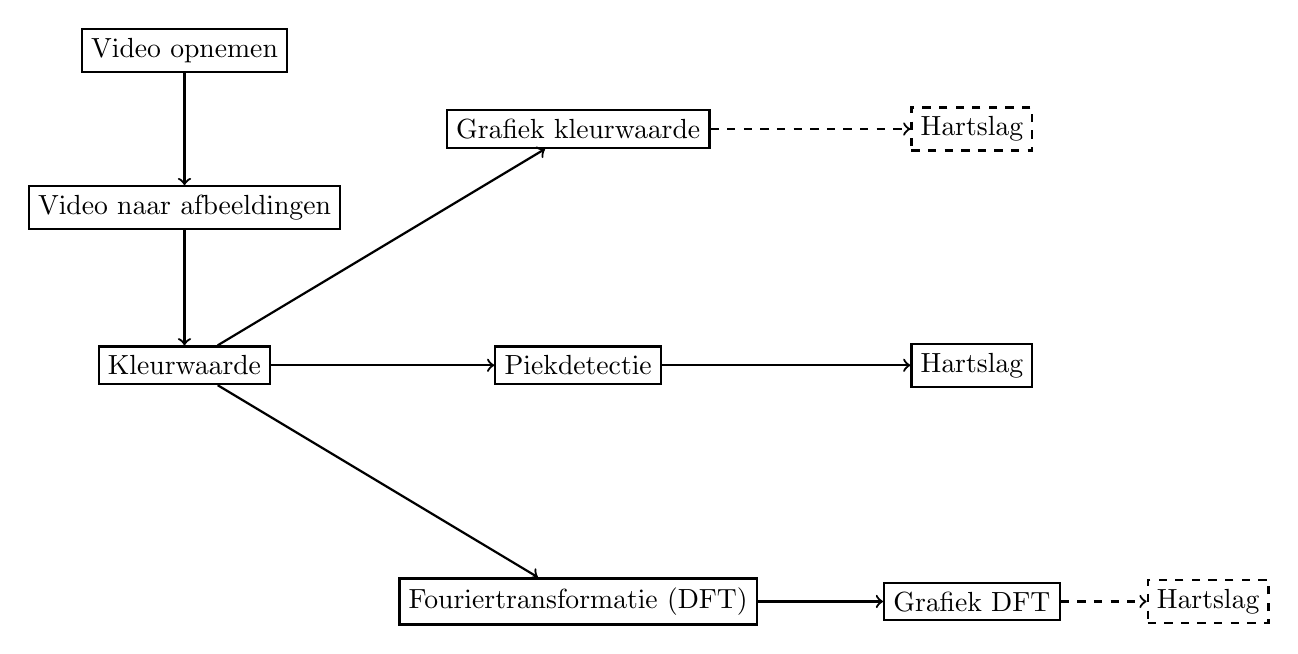
\begin{tikzpicture}[thick]
\node[draw,rectangle] at (0,0) (a) {Video opnemen};
\node[draw,rectangle] at (0,-2) (b) {Video naar afbeeldingen};
\node[draw,rectangle] at (0,-4) (c) {Kleurwaarde};
\node[draw,rectangle] at (5,-1) (d) {Grafiek kleurwaarde};
\node[draw,rectangle,dashed] at (10,-1) (j) {Hartslag};
\node[draw,rectangle] at (5,-4) (e) {Piekdetectie};
\node[draw,rectangle] at (10,-4) (f) {Hartslag};
\node[draw,rectangle] at (5,-7) (g) {Fouriertransformatie (DFT)};
\node[draw,rectangle] at (10,-7) (h) {Grafiek DFT};
\node[draw,rectangle,dashed] at (13,-7) (i) {Hartslag};

\draw[->] (a) -- (b) ;
\draw[->] (b) -- (c) ;

\draw[->] (c) -- (d) ;
\draw[->] (c) -- (e) ;
\draw[->] (c) -- (g) ;

\draw[->,dashed] (d) -- (j) ;
\draw[->] (e) -- (f) ;
\draw[->] (g) -- (h) ;
\draw[->,dashed] (h) -- (i) ;

\end{tikzpicture}

%\begin{tikzpicture}
%\sbEntree{n1}
%\sbRelier[RecordButton]{n1}
%\sbBlocL{n1}{Video opnemen}{n2}
%%\sbBlocL{n2}{Video naar afbeeldingen}{n3}
%%\sbBlocL{n3}{Kleurwaarde van afbeeldingen}{n4}
%%\sbBlocL{n4}{Grafiek van kleurwaarde ifv tijd}{n5}
%%\sbBlocL{n5}{Piekdetectie kleurwaarden}{}
%%\sbBlocL{n6}{Hartslag berekenen}{n7}
%%\sbSortie[5]{S1}{n7}
%%\sbNomLien[0.8]{S1}{$Hartslag$}
%
%%\sbEntree{E}
%%\sbComp{a}{E}
%%\sbBloc{b}{$H_1$}{a}
%%\sbRelier[$E_1$]{E}{a}
%%\sbBlocL{c}{$H_2$}{b}
%%\sbRelier[$\epsilon$]{a}{b}
%%\sbComph{d}{c}
%%\sbRelier[u]{c}{d}
%%\sbBlocL{e}{$H_3$}{d}
%%\sbBlocL{f}{$H_4$}{e}
%%\sbSortie[5]{S1}{f}
%%\sbRelier{f}{S1}
%%\sbNomLien[0.8]{S1}{$S_1$}
%%\sbDecaleNoeudy[-4]{f}{u}
%%\sbDecaleNoeudy{e}{v}
%%\sbBlocr{r1}{$R_1$}{u}
%%\sbBlocr{r2}{$R_2$}{v}
%%\sbBlocrL{r3}{$R_3$}{r2}
%%\sbRelieryx{f-S1}{r1}
%%\sbRelierxy[n1]{r1}{d}
%%\sbRelieryx{e-f}{r2}
%%\sbRelierxy[n2]{r3}{a}
%\end{tikzpicture}





%%%%%%%%%%%%%%%%%%%%%%%%%%%%%%%%%%%%%%%%%%%%%%%%%%%%%%%%%%%%%%%%%%%%%%%
%%%%%%%%%%%%%%%%%%%%%%%%%%%%%%%%%%%%%%%%%%%%%%%%%%%%%%%%%%%%%%%%%%%%%%%
\deelmetoef{Module 2}{Apps maken met MIT App Inventor 2}{Module 2. Apps maken met MIT App Inventor 2}{Oplossingen module 2}{Oplossingen module 2}
%%%%%%%%%%%%%%%%%%%%%%%%%%%%%%%%%%%%%%%%%%%%%%%%%%%%%%%%%%%%%%%%%%%%%%%
%%%%%%%%%%%%%%%%%%%%%%%%%%%%%%%%%%%%%%%%%%%%%%%%%%%%%%%%%%%%%%%%%%%%%%%

\begin{samenvatting}
De hartslagmonitor die we gaan maken is een smartphone app. MIT, een bekende universiteit in de Verenigde Staten, ontwikkelde een programmeeromgeving waarmee je zeer eenvoudig apps kan maken en testen. In dit hoofdstuk bespreken we de belangrijkste structuren voor het maken van een app. Ook in andere programmeertalen en -omgevingen zal je deze structuren kunnen gebruiken.
\end{samenvatting}
%

%%%%%%%%%%%%%%%%%%%%%%%%%%%%%%%%%%%%%%%%%%%%%%%%%%%%%%%%%%%%%%%%%%%%%%%
\section{MIT App Inventor 2}
\label{sec:Mod2_Sec1}
%%%%%%%%%%%%%%%%%%%%%%%%%%%%%%%%%%%%%%%%%%%%%%%%%%%%%%%%%%%%%%%%%%%%%%%
%
Met behulp van MIT App Inventor 2 kan je zelf apps maken. Alles wat je nodig hebt, is een computer met wifi-verbinding en een smartphone die met hetzelfde wifi-netwerk geconnecteerd is.

\subsection{Maken van de app}

Surf naar de website \url{http://appinventor.mit.edu/explore/} en klik rechtsboven op create apps! Je zal moeten inloggen met een google account. Als je nog geen google account hebt, kan je die aanmaken via \url{https://accounts.google.com/signup}. Na succesvol aanmelden kom je op de pagina met je projecten terecht. 

Cre\"eer een nieuw project, noem het bv \textquotedblleft HelloWorld\textquotedblright, en klik erop om het project te openen. 

Je komt op het startscherm terecht. Er zijn twee \textquoteleft views\textquoteright. De eerste view is de \emph{designer view}, weergegeven in Figuur \ref{fig:view_designer}.

\figuurmetlabel[\label{fig:view_designer}]{width=.8\linewidth}{module2/overviewAI}{Designer view in MIT App Inventor 2. Overschakelen tussen views doe je rechtsbovenaan (blauwe rechthoek). Tabs zijn aangeduid in rood.}

Hierin kan je de componenten toevoegen die je zal zien op het scherm tijdens het uitvoeren van je app. In de tab \emph{Palette} (links) vind je alle componenten die je kan toevoegen. Dit is bijvoorbeeld een knop (Engels: button), een label, een afbeelding (Engels: image) enz. Je voegt componenten toe door ze vast te nemen en ze naar het scherm van de afgebeelde smartphone te slepen. Componenten kan je groeperen m.b.v. \texttt{HorizontalArrangement}, \texttt{VerticalArrangement} of \texttt{TableArrangement}. Componenten kan je een naam geven onder de tab \emph{Components} door de component aan te klikken en op \emph{Rename} te drukken. In de tab \emph{Properties} (rechts) kan je de eigenschappen van de component veranderen: Welke tekst moet op de knop staan? Wat is de lettergrootte? Wil je de tekst in een andere kleur weergeven? ... Als je wilt weten wat een component doet, kan je het vraagteken naast de component in de tab \emph{Palette} aanklikken voor een korte uitleg.

De andere view is de \emph{blocks view}, weergegeven in Figuur \ref{fig:view_block}.

\figuurmetlabel[\label{fig:view_block}]{width=.8\linewidth}{module2/uitlegAI_blocks}{Block view in MIT App Inventor 2.}

Hierin voeg je de functionaliteit toe aan je app. Wat moet er gebeuren als je op de knop drukt? Misschien wil je de tekst in een label aanpassen, of wil je een andere afbeelding tonen. Er kan veel; wat je implementeert, hangt af van je verbeelding.

\begin{opdracht}{Experimenteren met MIT App Inventor 2}
Ga na wat je allemaal kan doen in de programmeeromgeving. Welke componenten bestaan er allemaal? Welke eigenschappen kan je aanpassen?

Probeer een eerste app te maken. De app bevat een knop met de tekst \textquotedblleft Zeg hallo\textquotedblright, en een label zonder tekst. Als je op de knop drukt, moet de tekst \textquotedblleft Hello world!\textquotedblright \ in het label verschijnen. Dit \textquotedblleft Hello world!\textquotedblright-programma is een van de simpelste programmatjes die je kan schrijven. Wanneer programmeurs een nieuwe programmeertaal aanleren, schrijven ze steeds \textquotedblleft Hello world!\textquotedblright-programma om te leren werken met de nieuwe taal, die we met een geleerder woord syntax noemen.
\end{opdracht}

\subsection{Testen en uitvoeren van de app}
Om de app te testen moet je de MIT App Inventor 2 Companion App (te vinden in de Google Play Store) installeren op je smartphone. 
Zorg ervoor dat je computer en smartphone met hetzelfde wifi-netwerk verbonden zijn. 
Klik op connect, rechtsboven in Figuur \ref{fig:view_designer}, en kies de eerste optie \textquotedblleft AI companion\textquotedblright. Er verschijnt een QR-code die je kan scannen met je smartphone met de MIT App Inventor 2 Companion App. De app opent op je smartphone, zodat je de werking van de app kan testen.

Als je smartphone geconnecteerd is via de Companion App, verandert de app op je smartphone mee wanneer je aanpassingen doet aan de componenten op het scherm. Soms werkt dit echter niet zo goed. Breek dan de connectie met de smartphone af via \texttt{Connection - reset connection} en maak de verbinding opnieuw via \texttt{Connection - AI companion}.

Als je de app die je ontworp getest hebt via de App Inventor 2 Companion App en de app aan de vereisten voldoet, kan je de app downloaden. Dan hoef je niet meer steeds de QR code te scannen als je de app wilt gebruiken. De app kan je installeren via \emph{Build - App (provide QR code for .apk)}. Door een QR code te scannen met je GSM kan je het installatie-bestand (.apk) downloaden op je smartphone. Wanneer je het .apk-bestand opent, installeert de app.

\begin{opdracht}{Good morning app}
	Toon \textquotedblleft Good morning!\textquotedblright \ in drie verschillende talen op het scherm, nl. Italiaans, Spaans en Duits.
	
	\begin{minipage}{.5\linewidth}
		\gewonefiguur{width=5cm}{module2/goedemorgenApp}
	\end{minipage}
	\begin{minipage}{.5\linewidth}
		\begin{enumerate}
			\item Cre\"eer een nieuw project.
			\item Ontwikkel de designer view:
			\begin{itemize}
				\item Welke layout?
				\item Welke componenten?
				\item Welke naam voor elke component?
				\item Welke eigenschappen voor elke component?
			\end{itemize}
			\item Ontwikkel de block view
			\begin{itemize}
				\item Indien klik op knopItaliaans: \textquotedblleft Buongiorno!\textquotedblright
				\item Indien klik op knopSpaans: \textquotedblleft Buenos dias!\textquotedblright
				\item Indien klik op knopDuits: \textquotedblleft Guten Morgen!\textquotedblright
			\end{itemize}
		\end{enumerate}
	\end{minipage}

Test de werking van je app grondig. Doet de app op elk moment wat je ervan verwacht? Indien niet: ga op zoek naar de onderliggende oorzaak. Dit proces, waarin je ongewenste fouten in de werking van de app opspoort en wegwerkt, heet \textquotedblleft debuggen \textquotedblright. Zelfs de beste programmeurs moeten hun apps debuggen. Dit is soms een frustrerend proces, maar het is helaas wel een wezenlijk onderdeel van programmeren.

\end{opdracht}

%%%%%%%%%%%%%%%%%%%%%%%%%%%%%%%%%%%%%%%%%%%%%%%%%%%%%%%%%%%%%%%%%%%%%%%
\section{Blokken in de blocks view}
\label{sec:Mod2_Sec2}
%%%%%%%%%%%%%%%%%%%%%%%%%%%%%%%%%%%%%%%%%%%%%%%%%%%%%%%%%%%%%%%%%%%%%%%
%
Met MIT App Inventor 2 kan je heel gemakkelijk zelf aan de slag. De betekenis van de componenten is vaak intu\"itief duidelijk en via het vraagteken kan je extra uitleg oproepen. 

Hieronder bespreken we enkele belangrijke blokken uit de blocks view, waarvan de bedoeling misschien iets minder vanzelfsprekend is.

\subsection{Controle (control)}
De meeste programmeertalen zijn opgebouwd rond drie belangrijke controlestructuren: \textquoteleft if\textquoteright-loops om beslissingen te nemen, en \textquoteleft for\textquoteright-loops en \textquoteleft while\textquoteright-loops om herhaling in te bouwen.

\subsubsection{Beslissingen nemen: \emph{If then} blok}

\begin{minipage}{.5\linewidth}
\gewonefiguur{width=7cm}{module2/if.jpg}
\end{minipage}
\begin{minipage}{.5\linewidth}
\gewonefiguur{width=7cm}{module2/ifStructures}
\end{minipage}

\textquoteleft If\textquoteright-lussen laten toe een programma dynamisch te maken. Een \textquoteleft If\textquoteright-lus kan je vergelijken met het kiezen van een weg op een kruispunt: als een voorwaarde voldaan is (YES), ga je naar links; anders ga je rechts. 

Het testen of een voorwaarde voldaan is, gebeurt met een \texttt{Boolean} expressie.
Een \texttt{Boolean} expressie is een uitdrukking die ofwel waar of ofwel vals is.
Het resultaat van \texttt{Boolean} expressie is een \texttt{Boolean}, een variabele die maar twee waarden kan aannemen: \texttt{true} als de voorwaarde voldaan is, en \texttt{false} als de voorwaarde niet voldaan is.

Je kan kiezen om een bewerking enkel uit te voeren als een voorwaarde voldaan is (\emph{If then} blok) of de ene bewerking uit te voeren als de voorwaarde voldaan is, en een andere als de voorwaarde niet voldaan is (\emph{If then else} blok). Als je echt complexe dingen wil doen, kan je extra voorwaarden toevoegen (\emph{If then, else if then, else then} blok).

\subsubsection{Herhaling: \emph{While test} lus of \emph{for each} lus}

Voor zaken die vaak uitgevoerd moeten worden, bv. de tekst op een label laten optellen van 1 tot 100, kan je gebruik maken van een repetitie-blok, zoals een \emph{While test} lus of \emph{for each} lus.

\gewonefiguur{width=\linewidth}{module2/repititionStructures2}

Bij een \emph{for each}-lus wordt een teller (in ons voorbeeld \texttt{number}) steeds verhoogd (in ons voorbeeld met $Z$) binnen een bereik van waarden (in ons voorbeeld tussen $X$ en $Y$). Een \emph{for}-lus is ideaal om een probleem op te lossen waarbij een lus een vast aantal keer herhaald moet worden.

Een \emph{While test} lus heeft twee delen: (1) een \emph{test}-socket: \texttt{Boolean} expressie (waar of niet waar?) die getest wordt, en (2) een \emph{do}-socket: een verzameling instructies die uitgevoerd wordt zolang de \texttt{Boolean} expressie \texttt{true} is. Pas op dat je geen oneindige lussen maakt: ooit moet de \texttt{Boolean} expressie \texttt{false} worden, anders blijf je vastzitten in de \emph{while}-lus.

\subsection{Logica (Logic)}

Zoals eerder gezegd is een \texttt{Boolean} expressie een expressie die ofwel waar of ofwel vals is.
Logische operatoren (zoals \texttt{AND} en \texttt{OR}) kunnen gebruikt worden om meerdere boolean expressies samen te stellen en zo meer complexe voorwaarden te testen. 

De logische operator \texttt{AND} geeft als output waar als beide inputs waar zijn, en onwaar als een of meerdere inputs onwaar zijn. 

De logische operator \texttt{OR} geeft als output waar als minstens een van beide inputs waar is, en onwaar als beide inputs onwaar zijn.

De logische operator \texttt{NOT} geeft als output onwaar als de input waar is en geeft als output waar als de input onwaar is.

\subsection{Wiskunde (Math)}
Uiteraard kunnen bewerkingen op getallen uitgevoerd worden. Je vindt het volledige overzicht van mogelijke bewerkingen onder \emph{Blocks - Math}.

\subsection{Tekst (Text)}
Naast wiskundige bewerkingen kan je ook tekst input van de gebruiker verwerken. De mogelijke bewerkingen die je op tekst kan uitvoeren vind je onder \emph{Blocks - Text}.

\subsection{Variabelen (Variables)}
Variabelen worden gebruikt om waarden bij te houden. Een bij te houden waarde kan bv. het resultaat van een wiskunde bewerking zijn, of een tekst input van de gebruiker die je later nog wilt aanpassen. 

Belangrijk is dat er een onderscheid gemaakt wordt tussen lokale en globale variabelen, zie Figuur \ref{fig:variabele}. Globale variabelen worden aangemaakt bij de opstart van het programma en kunnen doorheen het hele programma gebruikt worden. We zouden kunnen zeggen dat je vanuit elk blok \textquotedblleft aan de globale variabele kan\textquotedblright.
Lokale variabelen worden aangemaakt binnen een blok en kunnen enkel door blokken binnen de grenzen van de lokale variabele gebruikt worden. Je \textquotedblleft kan er dus enkel aan\textquotedblright \ binnen het oranje blok zelf. Vandaar dat het blok voor een lokale variabele onderaan nog een oranje staartje heeft. Dit staartje duidt aan binnen welke grenzen \textquotedblleft je aan de variabele kan\textquotedblright.

\figuurmetlabel[\label{fig:variabele}]{width=8cm}{module2/variabelen}{Het bovenste blok toont hoe je een globale variabele kan aanmaken, die doorheen het hele programma gebruikt kan worden. Het onderste blok toont hoe je een lokale variabele kan aanmaken, die enkel toegankelijk is binnen het blok van de variabele.}

De \texttt{Get}-instructies worden gebruikt om de waarde van een variabele op te halen. De \texttt{Set}-instructie wordt gebruikt om de waarde van een variabele te wijzigen.

\subsection{Lijsten (Lists)}
Een lijst kan meerdere items met gelijkaardige data bevatten. Zo kan je bijvoorbeeld een lijst van getallen hebben, of een lijst van tekstwaarden. Als je 100 getallen moet bijhouden, is het makkelijker een lijst te gebruiken dan 100 verschillende variabelen.

Nadat een lijst wordt aangemaakt zoals in Figuur \ref{fig:lijst}, kan je extra items aan de lijst toevoegen, of er items uit verwijderen. De volledige lijst van bewerkingen die je op een lijst kan toepassen, vind je onder \emph{Blocks - list}

\figuurmetlabel[\label{fig:lijst}]{width=8cm}{module2/lijst}{Je kan een lege lijst aanmaken (boven), of een lijst aanmaken die reeds een aantal elementen bevat.}



%%%%%%%%%%%%%%%%%%%%%%%%%%%%%%%%%%%%%%%%%%%%%%%%%%%%%%%%%%%%%%%%%%%%%%%
%%%%%%%%%%%%%%%%%%%%%%%%%%%%%%%%%%%%%%%%%%%%%%%%%%%%%%%%%%%%%%%%%%%%%%%
\deelmetoef{Module 3}{Digitale afbeeldingen en video}{Module 3. Digitale afbeeldingen en video}{Oplossingen module 3}{Oplossingen module 3}
\label{sec:digafbvid}
%%%%%%%%%%%%%%%%%%%%%%%%%%%%%%%%%%%%%%%%%%%%%%%%%%%%%%%%%%%%%%%%%%%%%%%
%%%%%%%%%%%%%%%%%%%%%%%%%%%%%%%%%%%%%%%%%%%%%%%%%%%%%%%%%%%%%%%%%%%%%%%

\begin{samenvatting}
Het meten van je hartslag met de smartphone is gebaseerd op kleurveranderingen in je vingertop, die we met de smartphone camera registreren in een video. Om goed te begrijpen hoe we die kleurveranderingen precies kunnen detecteren, is het belangrijk de basisprincipes achter digitale afbeeldingen en video te begrijpen. Daar gaan we in deze module dieper op in.
\end{samenvatting}
%

%%%%%%%%%%%%%%%%%%%%%%%%%%%%%%%%%%%%%%%%%%%%%%%%%%%%%%%%%%%%%%%%%%%%%%%
\section{Digitale afbeeldingen}
\label{sec:Mod3_Sec1}
%%%%%%%%%%%%%%%%%%%%%%%%%%%%%%%%%%%%%%%%%%%%%%%%%%%%%%%%%%%%%%%%%%%%%%%
%

\subsection{Hoe zijn digitale afbeeldingen opgebouwd?}

Om jullie te laten kennis maken met de basisprincipes achter digitale afbeeldingen, raden we jullie aan onderstaand filmpje te bekijken. Het is een Engelstalig filmpje, maar je kan het ondertitelen (in het Engels) en eventueel ook vertraagd bekijken.

\gewonefiguur{width=4cm}{module3/qrcode_youtubespreadsheets}

In het filmpje wordt uitgelegd dat digitale afbeeldingen opgebouwd zijn als een rooster. De vakjes uit het rooster noemen we \textquotedblleft pixels\textquotedblright. 

\gewonefiguur{width=.7\linewidth}{module3/voetballer-raster}

Elk pixel heeft een roodwaarde, een groenwaarde en een blauwwaarde. Met de combinatie van drie kleuren, nl. rood, groen en blauw, kan je quasi elke bestaande kleur genereren. 

De rood-, groen- en blauwwaarde van een pixel is steeds een getal tussen 0 en 255. Hoe kleiner het getal, hoe donkerder de kleur. Een roodwaarde van 0 komt dus overeen met een rood dat bijna zwart is. Omgekeerd: hoe groter het getal, hoe lichter de kleur. Een roodwaarde van 255 komt dus overeen met een rood dat bijna helemaal wit is. De drie getalwaarden voor rood, groen en zwart samen bepalen volledig de kleur die je zal zien. Dit drietal noemen we de RGB-waarde (R van rood/red, G van groen/green en B van blauw/blue) van de pixel.

\begin{oef}
	Hoeveel verschillende RGB-kleuren kan je genereren als de rood-, groen- en blauwwaarden steeds een waarde tussen 0 en 255 aannemen? 
\end{oef}
\oplos{Je kan $255 \cdot 255 \cdot 255 = 16 581 375$ verschillende kleuren genereren.}

Hieronder zie je hoe een digitale afbeelding in een computer voorgesteld wordt: van elk pixel wordt bijgehouden hoeveel rood, groen en blauw die bevat. 

\gewonefiguur{width=.7\linewidth}{module3/voetballer-opgesplitst_RGB}

Je kan ook zelf experimenteren met de RGB-waarden van een foto. 

Via \url{http://makeanddo4d.com/spreadsheet/} of onderstaande QR-code kan je een foto omzetten in een Excel-werkblad. Inzoomen in het werkblad toont je de RBG-waarden van de inviduele pixels. Uitzoomen in het werkblad toont je de volledige foto, weliswaar met een beperkte resolutie.

\gewonefiguur{width=4cm}{module3/qrcode_spreadsheetmaker}

\gewonefiguur{width=\linewidth}{module3/spreadsheetVb}

Als je de RGB waarden van enkele pixels aanpast en een beetje uitzoomt, zal je een andere kleur zien.


\subsection{Toepassing op de hartslagmonitor: roodwaarde berekenen in MIT App Inventor 2}

Voor de hartslagmonitor gaan we de roodwaarde van je vingertop analyseren. 

Gedurende 1 hartslag verandert je vingertop heel subtiel van kleur. 
Wanneer het bloed door je aders gepompt wordt, zetten je aders een heel klein beetje uit. Daardoor komt het bloed net iets dichter bij de oppervlakte van je huid en kleurt je vingertop net iets meer rood dan daarvoor.
Die verandering in roodwaarde van je vinger kan je met het blote oog niet detecteren, maar als je een filmpje maakt van je vinger, kan een computer, of zelfs je smartphone, die subtiele kleurverschillen wel waarnemen.

We maken een filmpje van onze vingertop. In dit filmpje worden de kleurveranderingen van je vingertop ten gevolge van je hartslag geregistreerd. Een filmpje dat afspeelt is in feite niet meer dan een aantal foto's die heel snel na elkaar getoond worden. Hier gaan we zo dadelijk, in Sectie \ref{sec:Mod3_Sec2} verder op in. Als we het opgenomen filmpje splitsen in de achterliggende foto's en van elke foto bepalen \textquotedblleft hoe rood\textquotedblright \  die is, kennen de roodwaarde van je vingertop in functie van de tijd. Dit is een grafiek, die net zoals de grafiek in hieronder (die je opmat via \emph{Science Journal}) een piek heeft voor elke hartslag. Door het aantal pieken in een beperkt tijdsinterval (bv $15~s$) te tellen en dit aantal te herleiden naar het aantal pieken per minuut (bv door het aantal pieken in $15~s$ te vermenigvuldigen met vier), kan je de hartslag berekenen.

\gewonefiguur{width=.3\linewidth}{module1/metingScienceJournal}

Om het project tot een goed einde te brengen, moeten we dus \textquotedblleft de roodwaarde\textquotedblright\  van een foto kunnen berekenen. 
De roodwaarde van een foto zullen we bepalen als het gemiddelde van de roodwaarde van elke pixel van de foto.


\begin{opdracht}{Opdracht: roodwaarde van een foto bepalen in App Inventor 2}
Bepaal de roodwaarde van een foto in App Inventor 2.

Volg daarvoor de volgende stappen:
\begin{enumerate}
	\item Voeg een \hl{canvas(E)/doek(NL)} component toe aan je scherm. 
	\item Upload een foto naar keuze en stel de foto in als achtergrond van het canvas.
	Pas de afmetingen van het canvas aan zodat de verhoudingen van de foto goed zijn. 
	
	\emph{Tip:} Voor de meeste rechtopstaande foto's is de verhouding tussen de hoogte en de breedte 16:9 (voor liggende foto's 9:16). Als de hoogte van een rechtopstaande foto vastgelegd wordt op 200 pixels, moet de breedte dus ongeveer $\frac{9}{16}200$ pixels zijn om de oorspronkelijke verhouding te respecteren.
	 
	\item Voeg een knop en een label component toe.
	
	\item Ga nu naar de \emph{Blocks view}. Voeg de nodige blokken toe zodat de gemiddelde roodwaarde van de foto berekend wordt als de knop ingedrukt wordt. De berekende roodwaarde verschijnt in de label component.
	
	\begin{itemize}
		\item \emph{Tip:} De canvas component heeft een methode/blok waarmee je de kleurwaarde van een pixel op breedte $x$ en hoogte $y$ in het rooster van de foto kan berekenen. 
		
		\item \emph{Tip:} Gebruik \hl{\texttt{Split color}} om de kleurwaarde van een foto op te splitsen in een lijst met drie elementen: de RGB-waarde.
		
		\item \emph{Tip:} Om de roodwaarde te bekomen, selecteer je het eerste element uit de lijst met de drie kleurwaarden. Je krijgt dus de R van de RGB-waarde.
		
		\item \emph{Tip:} Om de gemiddelde roodwaarde van een foto te berekenen, gebruik je twee for-lussen: \'e\'en lus loopt over alle pixels in de breedte van een foto ($x$ varieert), de andere lus loopt over alle pixels in de hoogte van de foto ($y$ varieert). De grenzen waarbinnen $x$ en $y$ vari\"eren, kan je bepalen a.d.h.v. de breedte en de hoogte van je canvas component.
		
		\item \emph{Tip:} om een gemiddelde van een rij getallen te berekenen, maak je eerst de som van alle getallen, en die som deel je vervolgens door het aantal getallen dat je opgeteld hebt:
		
		\begin{equation*}
		\text{Gemiddelde van 2, 7 en 10} = \frac{2+7+10}{3} = 6,33
		\end{equation*}
		
		Iets algemener, voor het gemiddelde van 5 willekeurige getallen:
		\begin{equation*}
		\overline{a_5} = \text{Gemiddelde van $a_1$, $a_2$, ..., $a_5$} = \frac{a_1+a_2+\ldots+a_5}{n} = \frac{\sum_{i=1}^{5} a_i}{5}
		\end{equation*}
		
		Nog algemener, voor het gemiddelde van $n$ willekeurige getallen:
		\begin{equation*}
		\overline{a_n} = \text{Gemiddelde van $a_1$, $a_2$, ..., $a_n$} = \frac{a_1+a_2+\ldots+a_n}{n} = \frac{\sum_{i=1}^{n} a_i}{n}
		\end{equation*}
		
	\end{itemize}

	\begin{opmerking}
		De gemiddelde roodwaarde van een foto berekenen kan even duren!
		
		Daarom gaan we in de toekomst niet werken via deze omslachtige manier, maar gebruiken we een apart blok dat een foto als input neemt en meteen de gemiddelde roodwaarde van de foto als output teruggeeft.
	\end{opmerking}
\end{enumerate}
\end{opdracht}

%%%%%%%%%%%%%%%%%%%%%%%%%%%%%%%%%%%%%%%%%%%%%%%%%%%%%%%%%%%%%%%%%%%%%%%
\section{Digitale video}
\label{sec:Mod3_Sec2}
%%%%%%%%%%%%%%%%%%%%%%%%%%%%%%%%%%%%%%%%%%%%%%%%%%%%%%%%%%%%%%%%%%%%%%%
%

In onderstaand filmpje (Engelstalig, met de mogelijkheid te ondertitelen en indien nodig te vertragen) worden de basisprincipes achter digitale video uitgelegd. 

\gewonefiguur{width=4cm}{module3/qrcode_youtubeDigitalVideo}

We vatten de inhoud van het filmpje hieronder nog even samen. Zoals eerder gezegd is digitale video een opeenvolging van digitale afbeeldingen, die snel na elkaar getoond worden met een vaste snelheid.
De digitale afbeeldingen waaruit een video is opgebouwd, noemen we frames.
De snelheid waarmee frames na elkaar getoond worden is de frame rate, uitgedrukt in frames per seconde (of kortweg $fps$).
Onderzoek heeft aangetoond dat een gemiddelde mens individuele afbeeldingen niet meer kan onderscheiden als ze op een snelheid van 24 $fps$ of sneller getoond worden.

\begin{oef}
	Hoelang is elke afbeelding zichtbaar als afbeeldingen in een video elkaar opvolgen aan een snelheid van 24 $fps$? 
	En wat als de frame rate 30 $fps$ is?
\end{oef}
\oplos{Voor een frame rate van 24 $fps$ wordt elke afbeelding gedurende 0.042 $s$ (of 42 $ms$) getoond. Voor een frame rate van 30 $fps$ wordt elke afbeelding gedurende 0.033 $s$ (of 33 $ms$) getoond.}

Elk frame heeft een breedte $B$ en een hoogte $H$, uitgedrukt in pixels.
We weten uit de vorige sectie dat een pixel in feite het kleinste bouwblokje van een digitale afbeelding is en dat elk pixel een RBG-waarde heeft.

\gewonefiguur{width=.7\linewidth}{module3/video_1}

De hoogte $H$ bepaalt de kwaliteit van het beeld. Hoe groter H, hoe scherper het beeld. Sommigen onder jullie hebben misschien al gehoord van standard definition (SD), high definition (HD) en full-HD beeldresolutie. 
De hoogte $H$ van de frames bepaalt of de beeldresolutie SD (als $H=480$ pixels), dan wel HD (als $H=720$ pixels), dan wel full-HD (als $H=1080$ pixels) is.

Encodering is een proces dat gebruikt wordt om de grootte van de video te reduceren m.b.v. wiskundige bewerkingen. Met de grootte van de video bedoelen we hoeveel ruimte nodig is op je computer of smartphone om de video op te slaan. De video-grootte wordt meestal uitgedrukt in megabytes (MB). Ongecomprimeerde video is video waarop geen encodering is toegepast en neemt veel geheugenruimte in op je smartphone of computer. Encodering past een wiskundige bewerking toe op je video die ervoor zorgt dat de geheugenruimte beperkt blijft, zonder de kwaliteit van de video te veel aan te tasten. Afhankelijk van de gebruikte wiskundige bewerkingen krijgen we een ander encoderingsformaat. Vaak gebruikte encoderingsformaten zijn .mp4 en .mov, maar er bestaan nog veel andere formaten.


\begin{opdracht}{Opdracht: een willekeurig filmpje splitsen in foto's}
Pluk een filmpje van het internet of maak zelf een filmpje. Gebruik de app \textquotedblleft Video naar afbeeldingen\textquotedblright \ om het filmpje te splitsen in opeenvolgende foto's. 

\begin{opmerking}
Het splitsen van video in afbeeldingen kan even duren!
\end{opmerking}

De foto's worden na het splitsen getoond. Deze foto's worden ook apart op de smartphone opgeslaan. De map waar de foto's worden opgeslaan wordt ook weergegeven. Je kan deze foto's dus ook achteraf nog raadplegen of gebruiken.

\end{opdracht}

Als je een willekeurig filmpje in foto's splitst, zie je hoe de foto's veranderen doorheen de tijd. Als de foto's snel genoeg na elkaar getoond worden, kan je oog de individuele foto's niet meer onderscheiden, waardoor je een continue beweging ziet.

\begin{opdracht}{Opdracht: een filmpje van je vingertop splitsen in foto's}
	Maak een filmpje van $15~s$ van de vingertop van je wijsvinger. Zet de flits van je smartphone aan. Leg je vinger op de lens van je camera en zorg dat je vinger de lens volledig bedekt. Het beeld zou volledig rood moeten zijn. Laat de camera gewoon rusten op je vingertop, je hoeft je vinger niet tegen de lens te duwen. 
	
	Splits het filmpje in foto's. 
	
	Zie jij de kleurverschillen ten gevolge van je hartslag?
\end{opdracht}


%%%%%%%%%%%%%%%%%%%%%%%%%%%%%%%%%%%%%%%%%%%%%%%%%%%%%%%%%%%%%%%%%%%%%%%
\section{Toepassing: de hartslagmonitor}
\label{sec:Mod3_Sec3}
%%%%%%%%%%%%%%%%%%%%%%%%%%%%%%%%%%%%%%%%%%%%%%%%%%%%%%%%%%%%%%%%%%%%%%%
%

\begin{opdracht}{Opdracht: roodwaarden bepalen en weergeven in MS Excel}
	In de vorige twee opdrachten hebben jullie een filmpje gemaakt van je vingertop en dit gesplitst in afzonderlijke afbeeldingen. Daarnaast hebben jullie geleerd hoe je in app inventor de roodwaarde van een individuele foto kan bepalen. Hier zullen we die twee combineren om de roodwaarden van de afzonderlijke foto's van je filmpje te bepalen. Die waarden slaan we op, en analyseren we in MS Excel, zodat we de hartslag kunnen berekenen.
	
\begin{enumerate}
	
	\item Maak een filmpje van $15~s$ van je vingertop of gebruik het filmpje uit de vorige opdracht.
	
	Zet de flits van je smartphone aan. Leg je vinger op de lens van je camera en zorg dat je vinger de lens volledig bedekt. Het beeld zou volledig rood moeten zijn. Laat de camera gewoon rusten op je vingertop, je hoeft je vinger niet tegen de lens te duwen.
	
	\item Splits het filmpje in foto's met de app \textquotedblleft Video naar afbeeldingen\textquotedblright.
	
	Als je dit in de vorige opdracht al gedaan hebt, mag je deze stap overslaan. Noteer de map waarin de afzonderlijke digitale afbeeldingen werden opgeslaan, dit heb je straks nodig.
	
	\item Maak een nieuw project aan in MIT App Inventor 2 en geef het een passende naam, bv \texttt{Hartslagmonitor\_redToExcel}. 
	
	\item Schrijf een app die, wanneer je de knop \emph{BerekenRoodwaarden} klikt, de roodwaarde van alle digitale afbeeldingen in de map berekent en toevoegt aan een lijst. Zet vervolgens deze lijst om naar een CSV-tabel en sla de tabel op op je smartphone.

	
%	\begin{oef}
		\begin{itemize}
			\item Voeg de knoppen/labels/\ldots die je denkt nodig te hebben toe aan je scherm.
			\item Wanneer de knop \emph{BerekenRoodwaarden} wordt ingedrukt, moet je de roodwaarden van alle afbeeldingen in de map bepalen. Maak daarom eerst een lijst van alle afbeeldingen die in de genoteerde map opgeslaan zijn. 
			
			Hiervoor moet je een extensie gebruiken: \emph{TaifunFile}. Voeg in de \emph{Designer}-view de extensie toe in de tab \emph{Palette} via \emph{Import extension}. Sleep de extensie dan naar het afgebeelde smartphone-scherm. De extensie zou onder de afgebeelde smartphone moeten verschijnen. 
			
			In de \emph{Blocks}-view gebruik je het blok \emph{TaifunFile - FileListAsync} om alle bestanden in de genoteerde map op te lijsten. Dit blok gaat alle bestanden in de gevraagde map \emph{directoryName} en met de gevraagde extensie \emph{extension} oplijsten. Als je bij \emph{includeSubDirectories} \texttt{true} zet, worden ook submappen meegenomen in de oplijsting. Als \emph{includeSubDirectories} \texttt{false} is, wordt enkel de map zelf bekeken. 

			De oplijsting is \emph{asynchroon}: dat wil zeggen dat de smartphone andere processen kan uitvoeren tijdens de oplijsting. Maar dat betekent ook dat we niet weten wanneer de bestanden opgelijst zijn. Daarom gebruiken we ook het blok \emph{TaifunFile - AfterFileListAsync}. Dit blok wordt geactiveerd wanneer alle bestanden opgelijst zijn, en dan kunnen we verder met onze berekeningen. Binnen dit blok hebben we een variabele \emph{fileList} waarin alle bestanden in de gevraagde map met de gevraagde extensie opgenomen zijn.
			
			Ga even na dat de bestanden in de gevraagde map correct opgelijst worden, door de variabele \emph{filelist} als label te tonen op het scherm van je smartphone. Ga pas verder naar de volgende stap als dit correct werkt.
			
			\item Je zal merken dat de bestanden niet noodzakelijk in numeriek oplopende volgende in \emph{fileList} staan. Daarom gaan we de lijst eerst sorteren. We willen immers eerst de roodwaarde van de eerste foto (met naam 001.jpg) berekenen, vervolgens van de tweede foto (met naam 002.jpg), enzovoort.
			
			Om de lijst te sorteren, hebben we een tweede extensie gemaakt: \emph{ListProcessing}. Voeg de extensie toe zoals voorheen via \emph{Import extension} en door de extensie naar het scherm van de afgebeelde smartphone te slepen.
			
			Gebruik het blok \emph{ListProcessing - SortList} om de lijst te sorteren. Ga na dat dit correct gebeurde door de bekomen lijst als label te tonen op het scherm van je smartphone. Ga pas verder naar de volgende stap als dit correct werkt.
			
			\item Itereer over de items/bestanden in de lijst met gesorteerde bestanden en bereken van elk bestand (en dus van elke afbeelding) de roodwaarde. Voeg de bekomen roodwaarden telkens toe aan een lijst, die je bijvoorbeeld \emph{redValueList} noemt.
			
			Ga even na dat de roodwaarden berekend worden, door de variabele \emph{redValueList} als label te tonen op het scherm van je smartphone. Ga pas verder naar de volgende stap als dit correct werkt.
			
			\item Ten slotte willen we de roodwaarden opslaan in een bestand dat we kunnen inlezen in MS Excel. Daarom moet de lijst omgezet worden in een CSV tabel. CSV staat voor \emph{Comma Separated Value}. Dit is een formaat dat vaak gebruikt wordt om gegevens op te slaan in een tekstbestand, dat eenvoudig kan ingelezen worden in MS Excel.
			
			Voeg een nieuwe \emph{File}-component toe aan je scherm. De component zou onder de afgebeelde smartphone moeten verschijnen. 
			
			Gebruik het blok \emph{File - SaveFile} en het blok \emph{List - list to csv table} om de lijst met roodwaarden (\emph{redValueList}) eerst om te zetten in een CSV tabel. Die CSV tabel is de \emph{text} input van het blok \emph{SaveFile}. De \emph{filename}-input mag je zelf kiezen, maar zorg dat de bestandsnaam eindigt op \textquotedblleft .csv\textquotedblright. Het csv-bestand zou moeten opgeslaan worden op je smartphone in de map AppInventor/data.
			
			Ga na dat het CSV-bestand inderdaad op de voorziene plaats en onder de voorziene naam opgeslaan is op je smartphone. Je kan navigeren door de bestanden op je smartphone via de app \textquotedblleft Bestanden\textquotedblright, die normaal gezien standaard ge\"installeerd is op Android smartphones.
			
			
		\end{itemize}
%	\end{oef}
%	\oplos{\begin{itemize}
%			\item Knop \emph{BerekenRoodwaarden}, 
%		\end{itemize}
	
	\item Kopieer het CSV-bestand van je smartphone naar je computer. Je kan dit doen door het bestand naar jezelf te mailen of het bestand op te laden naar je google drive en dan te downloaden vanaf je computer. Alternatief sluit je je smartphone aan op je computer via een USB-kabel en kopieer je het bestand rechtstreeks. 
	
	Het CSV-bestand bevat zoals gezegd de roodwaarden van de digitale afbeeldingen waaruit de video bestaat. Je kan deze waarden inlezen in MS Excel. 
	
	\begin{itemize}
		\item Open een nieuwe MS Excel werkmap.
		\item Lees de gegevens in via het tabblad \emph{Gegevens} - Van tekst. Verplaats de roodwaarden naar kolom B. Voeg bovenaan een lege rij toe en geef kolom B een passende titel.
		\item Voeg de tijdstippen toe in kolom A. 
		
		De eerste foto werd geregistreerd op tijdstip 0,00. Gebruik de frame rate om de registratietijden van de volgende foto's toe te voegen. Ga indien nodig even terug naar oefening 1 in Sectie \ref{sec:Mod3_Sec2} om de duurtijd per foto $d$ te berekenen a.d.h.v. de frame rate.
		
		Als je de frame rate niet kent, kan je die berekenen. Hiervoor moet je weten hoelang je filmpje duurt. Duid dit aan met $D$. Dit kan je zien op je smartphone. In MS Excel kan je nagaan hoeveel foto's ge\"extraheerd werden. Dit duid je aan met $N$. De totale duur van de video $D$ gedeeld door het aantal foto's in de video $N$ geeft je het aantal seconden per foto/frame $d=\frac{D}{N}$. 
		
		\item Geef kolom A een passende titel.
		
		\item Maak een grafiek die de roodwaarde in functie van de tijd weergeeft. Welke kolom levert de waarden die op de $x$-as komen? En welke gegevens komen op de $y$-as?
		
		Hieronder zie je een voorbeeld.
		
		\gewonefiguur{width=\linewidth}{module3/MSExcel_graphRedValues}
		
		\item Tel het aantal pieken in de grafiek. Noteer ook hoelang het filmpje duurde. Gebruik beide gegevens om de hartslag, het aantal pieken per minuut, te berekenen.
		
		In de grafiek hierboven tellen we 19 pieken op 15 seconden. De hartslag is dus $19 \cdot 4 = 76$ bpm.
		
		\item Als de grafiek niet mooi genoeg is om pieken te kunnen tellen, maak dan een nieuw filmpje en herhaal de bovenstaande stappen. 
		
		Ga na welke factoren (bv flits aan/uit, hoe hard je op de lens drukt, hoe je je vinger houdt, ...) de kwaliteit van de meting be\"invloeden. Hou hiermee rekening als je later nog pogingen onderneemt om de hartslag te meten. Schrijf indien nodig je bevindingen ergens op.
	\end{itemize}	

\end{enumerate}
	
\end{opdracht}

\begin{opdracht}{Opdracht: roodwaarden bepalen en weergeven in de app}
	In de vorige opdracht konden we voor het eerst onze hartslag bepalen o.b.v. een opgenomen video. De omweg via MS Excel is wel een beetje vervelend. In deze opdracht wijzigen we de app uit de vorige opdracht, zodat we de grafiek rechtstreeks in onze app kunnen maken en bekijken.
	
	\begin{enumerate}
		\item Kopieer het vorige project en geef het een passende naam, bv \texttt{Hartslagmonitor\_redToGraph}. 
		\item Om de tijd op de $x$-as correct te kunnen berekenen, moeten we de frame rate kennen. In de meeste nieuwe smartphones is de frame rate 30 $fps$. Dit is dus de standaardwaarde die we in de app zullen gebruiken.
		
		We moeten wel functionaliteit aan de app toevoegen die toelaat de frame rate te veranderen, mocht die niet overeenkomen met onze standaardwaarde van 30 $fps$. Voeg daarom een tekstinput \emph{fsInput} en een knop \emph{fsChanged} toe aan je app. Wanneer je de tekstinput verandert, moet je de op knop \emph{fsChanged} drukken, waarna een globale variabele \emph{fs} aangepast wordt.
		
		In de vorige opdracht berekende je de frame rate voor de smartphone die jij gebruikte. Ga na of je de standaardwaarde van 30 $fps$ inderdaad moet veranderen.
		
		\item Voeg een nieuwe knop \emph{plotValues} en een webviewer toe. Voeg ook de extensie \emph{Chartmaker} toe door de extensie te importeren en dan de componenten te slepen naar het afgebeelde smartphonescherm.
		
		Gebruik het blok \emph{Chartmaker - DrawLineGraph} om een lijngrafiek te maken. Je kan de grafiek een titel, $x$- en $y$-labels geven. De input $scalingFactor$ geeft aan met welke stapgrootte de waarden op de $x$-as veranderen. Dit is de duurtijd per foto $d$, die je in de vorige opdracht bepaalde. De input \emph{maxXValue} limiteert het bereik dat afgebeeld wordt op de $x$-as. Ten slotte moet je een label-naam meegeven, welke waarden je wilt uitzetten in de grafiek, en in welke webviewer je de grafiek wilt weergeven.
		
		Controleer dat de grafiek correct wordt weergegeven alvorens verder te gaan!
		
		\begin{opmerking}
			Als je geen internet connectie hebt, zal je de grafiek niet kunnen weergeven! 
		\end{opmerking}
	\end{enumerate}
\end{opdracht}
	



%%%%%%%%%%%%%%%%%%%%%%%%%%%%%%%%%%%%%%%%%%%%%%%%%%%%%%%%%%%%%%%%%%%%%%%
%%%%%%%%%%%%%%%%%%%%%%%%%%%%%%%%%%%%%%%%%%%%%%%%%%%%%%%%%%%%%%%%%%%%%%%
\deelmetoef{Module 4}{Automatische piekdetectie}{Module 4. Automatische piekdetectie}{Oplossingen module 4}{Oplossingen module 4}
\label{sec:piekdetectie}
%%%%%%%%%%%%%%%%%%%%%%%%%%%%%%%%%%%%%%%%%%%%%%%%%%%%%%%%%%%%%%%%%%%%%%%
%%%%%%%%%%%%%%%%%%%%%%%%%%%%%%%%%%%%%%%%%%%%%%%%%%%%%%%%%%%%%%%%%%%%%%%

\begin{samenvatting}
	In de vorige modules leerde je werken met App Inventor 2 en leerde je de basis van digitale afbeeldingen en video. In de slotopdracht van module 3 maakte je een grafiek waaruit je je hartslag kon afleiden door zelf pieken te tellen. In deze module gaan we na hoe de smartphone zelf die pieken kan detecteren, zodat wij van dat rekenwerk gespaard blijven. Daarvoor staan we stil bij wat een piek precies is, en hoe we de smartphone kunnen leren pieken te detecteren. 
\end{samenvatting}
%

%%%%%%%%%%%%%%%%%%%%%%%%%%%%%%%%%%%%%%%%%%%%%%%%%%%%%%%%%%%%%%%%%%%%%%%
\section{Wat is een piek in een signaal?}
\label{sec:Mod4_Sec1}
%%%%%%%%%%%%%%%%%%%%%%%%%%%%%%%%%%%%%%%%%%%%%%%%%%%%%%%%%%%%%%%%%%%%%%%
%
I.p.v. zelf pieken te tellen op een grafiek willen we dit automatisch doen in de app. Dit houdt in dat we de code moeten schrijven om pieken te detecteren. Door onze ervaringen in het dagelijkse leven kunnen wij mensen redelijk intu\"itief pieken herkennen. De smartphone daarentegen moet door ons gezegd worden wanneer hij een extra piek moet tellen. Daarom moeten we zelf ook even stilstaan bij wat een piek nu eigenlijk is.

\begin{steroef}
	Omschrijf in eigen woorden wat een piek is.
\end{steroef}
\oplos{Wellicht komen hier heel diverse antwoorden, afhankelijk van de achtergrond van de leerlingen. Leerlingen uit de 3e graad zullen wellicht over maxima spreken, terwijl leerlingen uit de 2e graad misschien meer woordelijke/minder wiskundige omschrijvingen zullen geven.}

Een woordelijke omschrijving van een piek hebben we gevonden, maar je smartphone redeneert wiskundiger. 

\begin{oef}
	Stel een wiskundige uitdrukking op die je in de code kan gebruiken om pieken te detecteren. 
	
	Hou er rekening mee dat je smartphone enkel een lijst met roodwaarden als input heeft. Die lijst kunnen we voorstellen als een verzameling $\{ u_1, u_2, u_3, \ldots, u_n \}$ met $n$ elementen, waarbij $u_i$ de $i$-de berekende gemiddelde roodwaarde voorstelt.
	
	Als je dit niet meteen ziet, kan je zelf een aantal voorbeeldlijsten maken en a.d.h.v. de vooorbeelden nagaan wanneer het signaal een piek bereikt.
\end{oef}
\oplos{Er is een maximum voor element $u_i$ als en slechts als: $u_i > u_{i-1}$ en $u_{i} < u_{i+1}$.}

\begin{opdracht}{Automatische piekdetectie in App Inventor 2}
Schrijf een app die automatisch pieken detecteert in een lijst. Hou bij (1) op welk volgnummer $i$ een piek $u_i$ gedetecteerd wordt, (2) hoeveel pieken in totaal gedetecteerd worden. Gebruik labels om die resultaten op je scherm weer te geven ter controle.

\begin{enumerate}
	\item Gebruik eerst een lijst die je zelf ingeeft met \emph{Lists - make a list}. Worden de pieken gedetecteerd op de plek die je verwacht? Pas je code aan tot je het verwachte resultaat bekomt.
	
	\item Gebruik nu een lijst met berekende roodwaarden, die we in de vorige module hebben opgeslaan in een CSV-bestand. Voeg daarom een \emph{File}-component toe je aan je app. Wanneer een knop \emph{Read CSV} ingedrukt wordt, moet het CSV-bestand die je opgeslaan hebt in de vorige module ingelezen worden. Kijk indien nodig even terug in je vorige project waar en onder welke naam je het CSV-bestand hebt opgeslaan. Als het CSV-bestand is ingelezen, moet de inhoud omgezet worden in een lijst en in een lijst geplaatst worden. Geef die lijst weer in een label en vergelijk de tekst met het CSV-bestand op een computer om te controleren dat dit correct gebeurde. 
	
	\item Gebruik de code uit stap 1 om automatisch pieken te detecteren in de lijst met roodwaarden. Komt dit overeen met het aantal pieken dat jij telt. Waarom (niet)?
	
	\begin{opmerking}
		Afhankelijk van het CSV-bestand dat je inleest, kan het zijn dat de lijst met roodwaarden in plaats van getallen als elementen lijsten met 1 element als elementen bevat. Om aan de roodwaarde te raken, moet je dan het eerste element halen uit elke lijst (die ook weer een element van de oorspronkelijke lijst is).
		
	%TODO indien onduidelijk tekening van Dimitri invoegen
	\end{opmerking}
	
	\begin{opmerking}
		Vaak is de lijst met roodwaarden een beetje \textquotedblleft ruizig\textquotedblright. Dit zorgt ervoor dat de app meer pieken detecteert dan wij zouden doen. Soms zien we een klein piekje in het signaal, dat we negeren, omdat het maar een kleine piek is, of omdat de piek te snel na een grote hartslagpiek komt. 
	\end{opmerking}

	\item We moeten de app dus leren dat sommige pieken moeten genegeerd worden, wanneer de piek niet echt hoog is, of heel snel komt. Hoe zou jij dit implementeren? Je hoeft dit niet meteen te doen, maar zorg wel dat je een plan hebt.
	
	\item De makkelijkste manier om de kleine piekjes te negeren is door de lijst met roodwaarden een beetje op te kuisen. De lijst met roodwaarden noemen we het signaal. De ruis die aanwezig is, is ongewenst. De ruis verandert vaak sneller dan het signaal zelf. Daardoor kunnen we de ruis verminderen door die snelle veranderingen weg te werken. Een eenvoudige manier om snelle veranderingen weg te werken is door opeenvolgende roodwaarden uit te middelen. Dit wordt ook wel laagdoorlaatfiltering genoemd: de snelle veranderingen, vaak ook hoge frequenties genoemd, worden weggefilterd uit het signaal.
	
	Schrijf code om opeenvolgende roodwaarden uit te middelen. Maak een nieuwe lijst, bv \emph{smoothRedValuesList}, waarin elk element een gemiddelde is van vier opeenvolgende elementen uit de originele lijst. Herinner je dat we een gemiddelde berekenen als een som van elementen, gedeeld door het aantal elementen dat opgeteld wordt.
	Voor het gemiddelde van 4 willekeurige getallen:
	\begin{equation*}
	\overline{a_4} = \text{Gemiddelde van $a_1$, $a_2$, $a_3$, $a_4$} = \frac{a_1+a_2+a_3+a_4}{4} = \frac{\sum_{i=1}^{4} a_i}{4}
	\end{equation*}
	
	\begin{opmerking}
		Tip: gebruik een \emph{for}-lus om de elementen van de nieuwe lijst \emph{smoothRedValuesList} te berekenen.
	\end{opmerking}

	\item Gebruik de code uit stap 1 om de pieken in de nieuwe lijst \emph{smoothRedValuesList} te berekenen. Bekom je een aanvaardbaar resultaat? Is het nodig meer of minder elementen van de originele lijst uit te middelen om tot een aanvaardbaar resultaat?
	
	\begin{opmerking}
	We spreken hier over een \emph{aanvaardbaar} resultaat en niet over een \emph{correct} resultaat. Het is goed mogelijk dat het aantal pieken dat je code detecteert licht afwijkt van het aantal pieken dat jij telt. Hoe sterk de afwijking is, hangt af van de kwaliteit van de opgenomen video. In Module 3 Sectie \ref{sec:Mod3_Sec3} gingen jullie al na welke factoren invloed hebben op de kwaliteit van de video.
	\end{opmerking}

	\item Als je tevreden bent over de automatische piekdetectie, kan je het aantal pieken gedetecteerd tijdens de duur van de video herleiden naar een waarde voor de hartslag, het aantal pieken per minuut.
	
	Gebruik de frame rate en het aantal elementen in de lijst met roodwaarden om de duur van de video te berekenen. Gebruik de regel van drie om het aantal pieken gedurende de videoduur te herleiden naar het aantal pieken per seconde. Dit is de gemeten hartslag. Geef die waarde weer in een label op het scherm. Bekom je een realistische waarde voor de gemeten hartslag?
\end{enumerate}
\end{opdracht}

%%%%%%%%%%%%%%%%%%%%%%%%%%%%%%%%%%%%%%%%%%%%%%%%%%%%%%%%%%%%%%%%%%%%%%%
\section{Intermezzo: differentiequoti\"ent}
\label{sec:Mod4_Sec2}
%%%%%%%%%%%%%%%%%%%%%%%%%%%%%%%%%%%%%%%%%%%%%%%%%%%%%%%%%%%%%%%%%%%%%%%
%
\emph{Bedoeld voor leerlingen uit de 3e graad.}

Voor de bepaling of een piek in het signaal bereikt wordt, maakte je gebruik van een wiskundige uitdrukking gerelateerd aan het differentiequoti\"ent.

Stel dat $\{ u_1, u_2, \ldots, u_n\}$ een signaal is, bv. een lijst met roodwaarden. 

\begin{opmerking}
	We noemen dit een \emph{discreet} signaal (in de figuur hieronder in rood aangeduid): de meetwaarden (bv roodwaarden) zijn slechts op bepaalde tijdstippen bepaald. 
	
	Naast \emph{discrete} signalen bestaan ook \emph{continue} signalen (in de figuur hieronder in zwart aangeduid), waarvoor op elk moment een meetwaarde beschikbaar is. Het signaal loopt dus - zoals de naam het zegt - continu door.
	
	\gewonefiguur{width=.5\linewidth}{module4/discreetvscontinu}
	
	Vaak spreekt men ook over \emph{digitale} en \emph{analoge} signalen. \emph{Digitale} signalen zijn vergelijkbaar met \emph{discrete} signalen, terwijl \emph{analoge} signalen te vergelijken zijn met \emph{continue} signalen, hoewel niet exact dezelfde zaken bedoeld worden met de termen \emph{digitaal/discreet} en \emph{analoog/continu}.

\end{opmerking}

\begin{oef}
	In de lessen wiskunde leerde je al over functies. Een grafiek van de functie met functievoorschrift $y=f(x)$ toont hoe de grootheid $y$ verandert i.f.v. de grootheid $x$. Vaak kan de grootheid $x$ een continu bereik van waarden aannemen. In dat geval spreken we over een discreet/continu signaal. \emph{(Schrap wat niet past.)}
\end{oef}
\oplos{Als de grootheid $x$ een continu bereik van waarden kan aannemen, spreken we over een continu signaal.}

De signalen waar we hier mee werken, kan je dus enigszins vergelijken met functies die je kent uit de wiskundelessen. 
Het verschil is dat we hier slechts op discrete momenten een functiewaarde kunnen bepalen, terwijl in de wiskundeles meestal met continue signalen gewerkt wordt.

We gaan terug naar ons discreet signaal $\{ u_1, u_2, \ldots, u_n\}$. De uitdrukking die je kan gebruiken om na te gaan of een piek bereikt was is:

\begin{equation*}
u_i-u_{i-1}
\end{equation*}

Immers, als $u_{i}-u_{i-1}>0$ en $u_{i+1}-u_{i}<0$ wordt een lokaal maximum, of een piek, bereikt op het tijdstip $i$.

Deze uitdrukking is sterk gerelateerd aan het differentiequoti\"ent $D$ voor een functie $f$:

\begin{equation}
D = \frac{f(a+\Delta h) - f(a)}{\Delta h}
\end{equation}

Voor zeer kleine waarden van $\Delta h$ benadert het differentiequoti\"ent de richtingsco\"effici\"ent van de raaklijn in het punt $(a,f(a))$. We zeggen ook weleens dat de afgeleide van de functie $f$ in het punt $(a,f(a))$ gelijk is aan 

\begin{eqnarray*}
f'(a) &=& \lim\limits_{\Delta h \to 0} D \\
&=& \lim\limits_{\Delta h \to 0} \frac{f(a+\Delta h)-f(a)}{\Delta h}
\end{eqnarray*}

Uit de wiskundelessen weet je dat een functie een extremum (= een maximum of een minimum) bereikt waar de afgeleide nul wordt. Om een \emph{minimum} te vinden zoeken we voor welke waarde(n) van $x$ de functie overgaat van dalend (afgeleide $f'(x)< 0$) naar dalend (afgeleide $f'(x)> 0$). Om een \emph{minimum} te vinden zoeken we voor welke waarde van $x$ de functie overgaat van stijgend (afgeleide $f'(x)>0$) naar dalend (afgeleide $f'(x)<0$).

Wat we in dit project doen, is zeer gelijkaardig: we kijken voor welke waarde van $i$ de waarde van $u_{i}-u_{i-1}$ overgaat van een positieve naar een negatieve waarde om een piek (= een maximum) te detecteren. 

\begin{oef}
	Nu we achterhaald hebben hoe onze aanpak in dit project vergelijkbaar is met afgeleiden en extrema-vraagstukken, kunnen we ons ook afvragen welke verschillen bestaan. Som op welke verschillen je ziet.
\end{oef}
\oplos{\begin{itemize}
		\item Bij afgeleiden gebruiken we continue signalen, en hier discrete.
		\item Bij afgeleiden is er nog een deling door $\Delta h$. Dit laten we hier achterwege. 
		 \begin{opmerking}
		 	Merk op dat je ook de uitdrukking $u_{i}-u_{i-1}$ zou kunnen delen door de tijdsduur tussen 2 foto's. Die tijdsduur is $\Delta i=1/fs$, het omgekeerde van de frame rate. 
		 	
		 	Die deling heeft geen invloed op het resultaat (de gedetecteerde pieken), omdat we zoeken voor welke waarde van $i$ de uitdrukking $u_{i}-u_{i-1}$ of $\frac{u_{i}-u_{i-1}}{\Delta i} = [ u_{i}-u_{i-1} ] fs$  overgaat van een positieve naar een negatieve waarde. Die extra (positieve) factor $fs$ be\"invloedt het teken, en dus ook de uitkomst, niet.
		 \end{opmerking}
	\end{itemize}}

%%%%%%%%%%%%%%%%%%%%%%%%%%%%%%%%%%%%%%%%%%%%%%%%%%%%%%%%%%%%%%%%%%%%%%%
\section{Intermezzo: Frequentieanalyse}
\label{sec:Mod4_Sec3}
%%%%%%%%%%%%%%%%%%%%%%%%%%%%%%%%%%%%%%%%%%%%%%%%%%%%%%%%%%%%%%%%%%%%%%%
%
\emph{Bedoeld voor leerlingen uit de 3e graad.}

Je zal al ondervonden hebben dat de nauwkeurigheid van de hartslagmeting afhangt van de kwaliteit van het opgenomen filmpje. Als je vingertop of de smartphone bewoog tijdens de opname, is de grafiek van de roodwaarde in functie van de tijd ruiziger. Hoe ruiziger het signaal, hoe moeilijker de detectie van pieken wordt. En hoe moeilijker de piekdetectie, hoe meer kans op fouten en hoe onnauwkeuriger de meting.

Er bestaat een andere manier om de hartslag te bepalen, die niet gebaseerd is op piekdetectie en daardoor iets nauwkeuriger is. Deze alternatieve manier is gebaseerd op frequentieanalyse.

\subsection{Geluid: zuivere en samengestelde tonen}

We nemen even afstand van onze hartslagmonitor. Om goed te kunnen uitleggen wat we met frequentieanalyse bedoelen, kijken we even naar geluid.

Geluid is een kleine verandering in luchtdruk, die zich door de lucht voortplant. Elk luchtdeeltje ondervindt een trilling en geeft die trilling door aan de luchtdeeltjes in zijn buurt. De trilling van een luchtdeeltje in functie van de tijd kan er uitzien zoals hieronder links.

\gewonefiguur{width=\linewidth}{module4/sinusTrilling}

De trilling hierboven (links) is een harmonische trilling, die als een sinusvormig signaal voorgesteld wordt en met als functievoorschrift 

\begin{equation*}
y(t) = A \sin(2\pi f t).
\end{equation*}

Links is de trilling voorgesteld in het tijdsdomein: de uitwijking in functie van de tijd is een sinusoidaal verloop. Rechts is de trilling voorgesteld in het frequentiedomein. Deze voorstelling noemen we dan ook het \emph{frequentiespectrum}. De frequentie van een trilling is gedefineerd als het aantal trillingen per seconde. De eenheid is $1/s$ of Hertz ($Hz$). Hoe het frequentiespectrum gevonden wordt, bespreken we later.

Deze trilling is een \emph{zuivere toon}: er is slechts 1 frequentie aanwezig. In het frequentiespectrum zien we maar 1 lijn. Het is het geluid dat je hoort als je een stemvork aanslaat.

\begin{oef}
\begin{itemize}
	\item Wat is de uitwijking, of amplitude $A$ van de trilling? 
	\item Hoe verandert het geluid als de amplitude verhoogt?
	\item Wat is de frequentie $f$ van de trilling? Vergeet de eenheid niet!
	\item Hoe verandert het geluid als de frequentie verhoogt?
	\item De periode is $T=1/f$ is het tijdsverschil tussen 2 opeenvolgende maximale (of minimale) uitwijkingen. Het is dus de tijd die 1 volledige trilling inneemt.
\end{itemize}
\end{oef}

Naast zuivere tonen bestaan ook samengestelde tonen. De meeste geluiden die je kent, zijn samengestelde tonen, waarin meerdere frequenties voorkomen. Hieronder zie je een voorbeeld.

\gewonefiguur{width=\linewidth}{module4/samengesteldeToon}

Het functievoorschrift van de afgebeelde trilling is 

\begin{equation*}
y(t) = 0.5 \sin(2 \pi 10 t) + 1 \sin(2 \pi 20 t) + 1 \sin(2 \pi 30 t).
\end{equation*}

De amplitude en frequentie van de samengestelde toon kan je uit het functievoorschrift afleiden: $A_1 = 0.5$, $f_1 = 10$ Hz, $A_2 = 1$, $f_2 = 20$ Hz, $A_3 = 1$ en $f_3 = 30$ Hz. Uit de linkergrafiek in het tijdsdomein kunnen die grootheden echter niet zo eenvoudig afgeleid worden. Gelukkig toont het frequentiespectrum ons wel de nodige informatie: er zijn drie zuivere trillingen, \'e\'en op 10 Hz met amplitude 0.5, \'e\'en op 20 Hz met amplitude 1 en \'e\'en op 30 Hz met amplitude 1.

In het algemeen kan een samengestelde toon geschreven worden als een som van $N$ zuivere tonen, elk met amplitude $A_n$ en frequentie $f_n$:

\begin{equation*}
y(t) = \sum_{n=1}^{N} A_n \sin(2 \pi f_n t).
\end{equation*}

\subsection{Frequentieanalyse: het idee van Fourier}

Meer algemeen kan je om het even welk periodiek signaal opbouwen door sinussen met veelvouden van een bepaalde grondfrequentie $f_0$ en verschillende amplituden op te tellen. Naarmate je meer termen optelt, krijgt het signaal een strakkere vorm.

Je kan elk periodiek signaal dus schrijven als een reeks

\begin{equation*}
y(t) = a_0 + \sum_{k=1}^{\infty} (a_k \cos(2 \pi k f_0 t) + b_k \sin(2 \pi k f_0 t)).
\end{equation*}

Frequentieanalyse of fourieranalyse is het ontleden van een oneindig lang periodiek signaal in de verschillende frequentiecomponenten waaruit het bestaat. 

Fourieranalyse bestaat er dus in de co\"effici\"enten $a_0$, $a_k$ en $b_k$ te zoeken, die bij elke frequentie $k f_0$ horen.

%TODO uitleg hoe dit te berekenen. Halen uit JC CI.

Fourieranalyse op geluidsignalen toont ons welke frequenties in een geluid voorkomen.

\subsection{Toepassing: fourieranalyse voor onze hartslagmonitor}

Terug naar onze hartslagmonitor. Wij zijn op zoek naar onze hartslag: het aantal keer dat ons hart klopt per minuuut. Dit is eigenlijk ook een soort van frequentie: het kloppen van ons hart kunnen we vergelijken met een geluidstrilling. Elke keer ons hart samentrekt, bevindt het bloed in onze vingertop zich iets verder van de huid en is de roodwaarde in onze video minimaal. En elke keer ons hart maximaal uitgezet is, bevindt het bloed in onze vingertop zich iets dichter bij huid en is de roodwaarde in onze video maximaal. Onze hartslag is dus de frequentie waarmee ons hart klopt en is meteen ook de frequentie waarmee de roodwaarde in de opgenomen video fluctueert. Als we dus het frequentiespectrum van ons roodwaarde-signaal kunnen opstellen, kunnen we uit de pieken hierin de hartslag afleiden.

\begin{opdracht}{Fourieranalyse in App Inventor 2}
Gebruik Fourieranalyse om de hartslag in een roodwaarde signaal te bepalen.
	
\begin{itemize}
	
	\item Maak een nieuw project \texttt{IL\_hartslagmonitor\_fourieranalyse}.
	
	\item Voorzie een aantal knoppen: \emph{readCSV}, \emph{calculateFFT} en \emph{plotFFT}. Voorzie ook een textbox waarin de gebruiker de frame rate ($fs$) kan aanpassen en een knop \emph{fsChanged} waarmee de gebruiker kan aangeven dat hij de frame rate aangepast heeft. Als de knop \emph{fsChanged} aangeklikt wordt, moet een globale variabele aangepast worden aan de inhoud van de textbox.
	
	\item Gebruik nu een lijst met berekende roodwaarden, die we in de vorige module hebben opgeslaan in een CSV-bestand. Gebruik zoveel mogelijk code uit vorige opdrachten. Voeg daarom een \emph{File}-component toe je aan je app. Wanneer een knop \emph{Read CSV} ingedrukt wordt, moet het CSV-bestand dat je opgeslaan hebt in de vorige module ingelezen worden. Kijk indien nodig even terug in je vorige project waar en onder welke naam je het CSV-bestand hebt opgeslaan. Als het CSV-bestand is ingelezen, moet de inhoud omgezet worden in een lijst en in een lijst geplaatst worden. Geef die lijst weer in een label en vergelijk de tekst met het CSV-bestand op een computer om te controleren dat dit correct gebeurde. 
	
	\item Kopieer de code uit een van de vorige opdrachten om opeenvolgende roodwaarden uit te middelen. Maak een nieuwe lijst, bv \emph{smoothRedValuesList}, waarin elk element een gemiddelde is van vier opeenvolgende elementen uit de originele lijst. 
	
	\begin{opmerking}
		Afhankelijk van het CSV-bestand dat je inleest, kan het zijn dat de lijst met roodwaarden in plaats van getallen als elementen lijsten met 1 element als elementen bevat. Om aan de roodwaarde te raken, moet je dan het eerste element halen uit elke lijst (die ook weer een element van de oorspronkelijke lijst is).
		
		%TODO indien onduidelijk tekening van Dimitri invoegen
	\end{opmerking}
	
 	\item De implementatie van de Fourieranalyse hebben we al voor jullie gedaan. Voeg daarom de extensie \emph{FFTCalculator} toe aan je app.
 	
	\item Gebruik het blok \emph{FFTCalculator - CalculateFft} om een Fourieranalyse uit te voeren wanneer de knop \emph{calculateCSV} aangeklikt wordt. Het resultaat is een lijst \emph{redValuesFFT}. 
	
	\item Verwijder het eerste element uit de lijst. Dit is nodig om een correct frequentiespectrum te kunnen maken.
	
	\item Wanneer op de knop \emph{plotFFT} gedrukt wordt, moet het frequentiespectrum getoond worden. Gebruik hiervoor het blok \emph{Chartmaker - DrawLineGraph}. Voeg opnieuw een \emph{Webviewer} toe aan je app. De titel van de grafiek en van de assen en het label kies je zelf. Maak de grafiek eerst met \emph{scalingFactor} gelijk aan 1.
	
	\item Op de $x$-as staan de mogelijke hartslagfrequenties. De sprong tussen twee opeenvolgende hartslagfrequenties is $\frac{60 \cdot fs}{\text{aantal roodwaarden}}$. Pas de \emph{scalingFactor} hieraan aan.

	
	\item Welke hartslag meten we nu op? De grootste piek in de grafiek toont welke frequentie \textquotedblleft het meeste in het signaal aanwezig is\textquotedblright. De $x$-waarde van de grootste piek toont dus de meest waarschijnlijke hartslag. Je kan de $x$- en $y$- waarde van een punt op de grafiek zien door erop te klikken. Komt de hoogste piek overeen met de hartslag die je zelf berekende? En met de hartslag die je app berekende via automatische piekdetectie?

	
	\begin{opmerking}
		Het is mogelijk dat de grootste piek zichtbaar is voor een heel kleine $x$-waarde. In dat geval is de piek wellicht veroorzaakt door ruis in het signaal. Komt de 2e grootste piek wel in de buurt bij een meer waarschijnlijke hartslag?
	\end{opmerking}

	Voor de roodwaarden in het voorbeeld CSV-bestand zou je een grafiek moeten zien zoals hieronder: 
	
	\gewonefiguur{width=\linewidth}{module4/redValuesFFT}
	
	In dit geval is de meest waarschijnlijke hartslag ongeveer 75 bpm.
	
	\item Wat is de stapgrootte waarmee de frequenties op de $x$-as verspringen? Wat zegt dit over de nauwkeurigheid van de hartslagmeting? Heeft de stapgrootte verband met een variabele die we eerder al gebruikten? Welke? Hoe kan je de nauwkeurigheid van de hartslagmeting verbeteren?
\end{itemize}
\end{opdracht}







%%%%%%%%%%%%%%%%%%%%%%%%%%%%%%%%%%%%%%%%%%%%%%%%%%%%%%%%%%%%%%%%%%%%%%%
%%%%%%%%%%%%%%%%%%%%%%%%%%%%%%%%%%%%%%%%%%%%%%%%%%%%%%%%%%%%%%%%%%%%%%%
\deelmetoef{Module 5}{Bouwen van de complete app}{Module 5. Bouwen van de complete app}{Oplossingen module 5}{Oplossingen module 5}
%%%%%%%%%%%%%%%%%%%%%%%%%%%%%%%%%%%%%%%%%%%%%%%%%%%%%%%%%%%%%%%%%%%%%%%
%%%%%%%%%%%%%%%%%%%%%%%%%%%%%%%%%%%%%%%%%%%%%%%%%%%%%%%%%%%%%%%%%%%%%%%

\begin{samenvatting}
\end{samenvatting}
%

%%%%%%%%%%%%%%%%%%%%%%%%%%%%%%%%%%%%%%%%%%%%%%%%%%%%%%%%%%%%%%%%%%%%%%%
\section{Video opnemen}
\label{sec:Mod5_Sec1}
%%%%%%%%%%%%%%%%%%%%%%%%%%%%%%%%%%%%%%%%%%%%%%%%%%%%%%%%%%%%%%%%%%%%%%%
%

%%%%%%%%%%%%%%%%%%%%%%%%%%%%%%%%%%%%%%%%%%%%%%%%%%%%%%%%%%%%%%%%%%%%%%%
\section{Video naar afbeeldingen m.b.v. app VideoNaarAfbeeldingen}
\label{sec:Mod5_Sec2}
%%%%%%%%%%%%%%%%%%%%%%%%%%%%%%%%%%%%%%%%%%%%%%%%%%%%%%%%%%%%%%%%%%%%%%%
%

%%%%%%%%%%%%%%%%%%%%%%%%%%%%%%%%%%%%%%%%%%%%%%%%%%%%%%%%%%%%%%%%%%%%%%%
\section{Gemiddelde roodwaarde voor elke afbeelding berekenen}
\label{sec:Mod5_Sec3}
%%%%%%%%%%%%%%%%%%%%%%%%%%%%%%%%%%%%%%%%%%%%%%%%%%%%%%%%%%%%%%%%%%%%%%%
%

%%%%%%%%%%%%%%%%%%%%%%%%%%%%%%%%%%%%%%%%%%%%%%%%%%%%%%%%%%%%%%%%%%%%%%%
\section{Grafiek van de gemiddelde roodwaarde i.f.v. de tijd}
\label{sec:Mod5_Sec4}
%%%%%%%%%%%%%%%%%%%%%%%%%%%%%%%%%%%%%%%%%%%%%%%%%%%%%%%%%%%%%%%%%%%%%%%
%

%%%%%%%%%%%%%%%%%%%%%%%%%%%%%%%%%%%%%%%%%%%%%%%%%%%%%%%%%%%%%%%%%%%%%%%
\section{Automatische piekdetectie en berekening van de hartslag}
\label{sec:Mod5_Sec5}
%%%%%%%%%%%%%%%%%%%%%%%%%%%%%%%%%%%%%%%%%%%%%%%%%%%%%%%%%%%%%%%%%%%%%%%
%

%%%%%%%%%%%%%%%%%%%%%%%%%%%%%%%%%%%%%%%%%%%%%%%%%%%%%%%%%%%%%%%%%%%%%%%
\section{Extra: frequentie-analyse m.b.v. Fouriertransformatie}
\label{sec:Mod5_Sec6}
%%%%%%%%%%%%%%%%%%%%%%%%%%%%%%%%%%%%%%%%%%%%%%%%%%%%%%%%%%%%%%%%%%%%%%%
%


%%%%%%%%%%%%%%%%%%%%%%%%%%%%%%%%%%%%%%%%%%%%%%%%%%%%%%%%%%%%%%%%%%%%%%%
%%%%%%%%%%%%%%%%%%%%%%%%%%%%%%%%%%%%%%%%%%%%%%%%%%%%%%%%%%%%%%%%%%%%%%%
\deelmetoef{Module 6}{Experimenteren met de app}{Module 6. Experimenteren met de app}{Oplossingen module 6}{Oplossingen module 6}
%%%%%%%%%%%%%%%%%%%%%%%%%%%%%%%%%%%%%%%%%%%%%%%%%%%%%%%%%%%%%%%%%%%%%%%
%%%%%%%%%%%%%%%%%%%%%%%%%%%%%%%%%%%%%%%%%%%%%%%%%%%%%%%%%%%%%%%%%%%%%%%

\begin{samenvatting}
\end{samenvatting}
%

%%%%%%%%%%%%%%%%%%%%%%%%%%%%%%%%%%%%%%%%%%%%%%%%%%%%%%%%%%%%%%%%%%%%%%%
\section{Vergelijking met bloeddrukmeter/hartslagmeter/smartwatch}
\label{sec:Mod6_Sec1}
%%%%%%%%%%%%%%%%%%%%%%%%%%%%%%%%%%%%%%%%%%%%%%%%%%%%%%%%%%%%%%%%%%%%%%%
%

%%%%%%%%%%%%%%%%%%%%%%%%%%%%%%%%%%%%%%%%%%%%%%%%%%%%%%%%%%%%%%%%%%%%%%%
\section{Invloed van sport en rust}
\label{sec:Mod6_Sec2}
%%%%%%%%%%%%%%%%%%%%%%%%%%%%%%%%%%%%%%%%%%%%%%%%%%%%%%%%%%%%%%%%%%%%%%%
%

%%%%%%%%%%%%%%%%%%%%%%%%%%%%%%%%%%%%%%%%%%%%%%%%%%%%%%%%%%%%%%%%%%%%%%%
\section{Evaluatie: wat kan beter?}
\label{sec:Mod6_Sec3}
%%%%%%%%%%%%%%%%%%%%%%%%%%%%%%%%%%%%%%%%%%%%%%%%%%%%%%%%%%%%%%%%%%%%%%%
%

%%%%%%%%%%%%%%%%%%%%%%%%%%%%%%%%%%%%%%%%%%%%%%%%%%%%%%%%%%%%%%%%%%%%%%%%%


%% Hier eindigt je eigenlijke LaTeX-file.

%% Van de volgende regel moet je afblijven.

\sluitfiles

%% Vervolgens kies je \'{e}\'{e}n van de onderstaande blokken, zonder iets aan deze blokken te veranderen:
%% ofwel produceer je achteraan de oplossingen van de oefeningen zonder ster; ofwel produceer je achteraan alle oplossingen.

%% Begin van het blok voor de oplossingen zonder ster %%

\deelzonderoef{}{Oplossingen van de oefeningen zonder $\ast$}{Oplossingen van de oefeningen zonder $\ast$}

\renewcommand{\sectionmark}[1]{\markright{\mijnoplosmark}}
\setcounter{secnumdepth}{0}
\titleformat{\section}[block]{}{}{0pt}{\zondernummer{#1}}

\input{inputs/oplossingen-zonder-ster.tmp}
%% Einde van het blok voor de oplossingen zonder ster %%

%% Begin van het blok voor alle oplossingen%%

\deelzonderoef{}{Oplossingen van alle oefeningen}{Oplossingen van alle oefeningen}

\renewcommand{\sectionmark}[1]{\markright{\mijnoplosmark}}
\setcounter{secnumdepth}{0}
\titleformat{\section}[block]{}{}{0pt}{\zondernummer{#1}}

\input{inputs/oplossingen-alle.tmp}
%% Einde van het blok voor alle oplossingen%%

%% In de volgende en laatste regel importeer je de achterflap. Je maakt een keuze tussen:
%% \includepdf{inputs/achterflap-leerling.pdf}
%% \includepdf{input/achterflap-leraar.pdf}
\includepdf{inputs/backcover.pdf}

\end{document} 